\documentclass[11pt,a4paper]{article}
\usepackage[margin=2.35cm]{geometry}
\usepackage{setspace}
\setstretch{1.22}
\usepackage{amsmath,amssymb}
\usepackage{booktabs}
\usepackage{tikz}
\usetikzlibrary{arrows.meta}
\usepackage[hidelinks]{hyperref}
\setlength{\parskip}{0.32em}
\setlength{\parindent}{1.05em}

\title{Identifying Thresher Operating Status\\from a Designed Sensor Placement}
\author{A short computer-science paper on the status model\\of a thesis on thresher efficiency}
\date{}

\begin{document}
\maketitle
\thispagestyle{empty}

\begin{abstract}
\noindent
Operating status of an axial thresher is a label of the running load, not a name for the crop. This paper treats status identification as a placement problem followed by a classifier. Eight axial stations are candidates. A \(D\)-optimal design for a quadratic load shape installs four of them: the inlet, two central bands, and the discharge. Window statistics from those stations, together with a few scalar channels that do not see the shape, form the feature vector. A feedforward network with one softmax output reaches \(89.8\%\) accuracy and macro-F1 \(0.846\) on a held-out mixture, against \(82.6\%\) and \(0.734\) for a linear softmax on the same features. Front-loaded recall rises from \(0.56\) to \(0.79\), and under-filled recall from \(0.27\) to \(0.61\). Accuracy saturates once the two end stations are present. The middle stations are kept because they identify curvature, not because they create another class. The numbers are a numerical experiment on a reduced-order plant.
\end{abstract}

\section{Introduction}

A thresher frees grain and then has to get the grain out of the straw. An axial machine keeps the crop in the cage long enough that the load has a shape: heavy at the inlet, lighter at the discharge if grain has been leaving along the way. The status an operator would name---stable, front-loaded, under-filled, at risk of a blockage, or simply losing too much grain---is a function of that shape and of the loss, not of a photograph of the grain. Surveys of learning in agriculture are dominated by perception tasks, and surveys of combine control are dominated by single actuator loops \cite{kamilaris2018,liakos2018,chen2025}. Impact sensors make sieve loss observable \cite{liang2016,zhao2011}. They do not decide which stations along the cage are worth reading, and they do not separate a front-loaded mat from a uniformly heavy one.

This paper is the status half of a computer-science thesis. The companion paper maps the same features to commands. Here the only product is the label. The plant is a reduced-order simulator used to assign labels and to corrupt sensors. It is not a field trial.

\section{Status, shape, and features}

Labels are assigned from the noise-free plant in a fixed priority. Blockage-risk wins if the peak station is at least \(0.84\times 1680\,\mathrm{N}\). High-loss wins if grain loss is at least \(2.8\%\). Front-loaded wins if the inlet exceeds the discharge by at least \(0.38\) of the mean load and the peak is at least \(760\,\mathrm{N}\). Under-filled wins if the mean load is at most \(430\,\mathrm{N}\). Anything else is stable. The classifier does not see this full vector. It sees a subset of the stations.

The design model on the normalized axis \(\xi\in[0,1]\) is the quadratic
\begin{equation}
F(\xi)=\theta_0+\theta_1\xi+\theta_2\xi^2+\varepsilon,
\qquad
\phi(\xi)=(1,\xi,\xi^2)^\top.
\label{eq:shape}
\end{equation}
A placement \(p\) has Fisher information \(M(p)=\sum_{i\in p}\phi(\xi_i)\phi(\xi_i)^\top\) under equal, independent noise \cite{atkinson2007}. The \(D\)-criterion maximizes \(\det M\). Fewer than three stations make \eqref{eq:shape} singular, so the two-station design uses the line \((1,\xi)\) and returns the two ends. The quadratic designs are stations \(\{1,4,8\}\) at three sensors, \(\{1,4,5,8\}\) at four, and \(\{1,2,4,5,8\}\) at five, numbering from the inlet. The installed set is the four-station design. Figure~\ref{fig:stations} marks it.

\begin{figure}[ht]
\centering
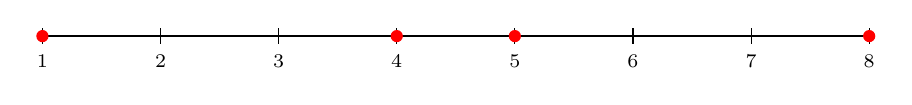
\begin{tikzpicture}[>=Stealth]
  \draw[thick] (0,0) -- (10.5,0);
  \foreach \i/\x in {1/0,2/1.5,3/3,4/4.5,5/6,6/7.5,7/9,8/10.5} {
    \draw (\x,0.1) -- (\x,-0.1);
    \node[below,font=\scriptsize] at (\x,-0.12) {\i};
  }
  \foreach \x in {0,4.5,6,10.5} {\fill[red] (\x,0) circle (2.2pt);}
\end{tikzpicture}
\caption{Candidate stations and the installed set \(\{1,4,5,8\}\).}
\label{fig:stations}
\end{figure}

Each installed station contributes the mean and the standard deviation of an eight-sample window. The means also contribute their coefficient of variation, the contrast between the first and the last installed station, and the maximum. Torque, housing vibration, a sieve-loss proxy, return flow, and shaft power contribute a mean and a deviation each. Moisture and feed contribute one reading each. Housing vibration in the simulator depends on intensity, moisture, and throughput, and not on which station is hot. Torque sees the level and not the location. If either scalar contained the contrast, the placement would be fake. With four stations the feature dimension is \(23\), after the scalings that put loads near unit magnitude. Inputs are then standardized with the training mean and variance.

Station noise is Gaussian with standard deviation \(22\,\mathrm{N}\). The scalar noises are fixed at the same values as the thesis and are not retuned against the test set.

\section{Classifier}

The network is feedforward, sizes \(23\)--\(48\)--\(32\)--\(5\), ReLU hidden units, softmax output, He-style initialization, and Adam at learning rate \(8\times 10^{-4}\) for \(100\) epochs \cite{he2015,kingma2015,goodfellow2016}. The epoch kept is the best validation accuracy, epoch \(99\). There are \(2885\) parameters. The baseline is a linear softmax on the same standardized features, with a small \(\ell_2\) penalty \cite{bishop2006}.

Disturbances are \(1600\) for training, \(350\) for validation, and \(500\) for test, seed \(7\), with feed and moisture spread over the working range and with wet-heavy and light corners enriched so the rare labels exist. Each disturbance is observed under a fixed command, under a moisture card, and under a random command. The test mixture has \(1500\) windows: \(614\) stable, \(397\) high-loss, \(221\) blockage-risk, \(212\) front-loaded, and \(56\) under-filled. Labels are computed from the clean plant at the command that generated the window.

\section{Results}

\begin{table}[ht]
\centering
\caption{Test windows, installed placement. Recall is omitted for the stable class, where both models sit near \(0.93\).}
\label{tab:status}
\begin{tabular}{@{}lcccccc@{}}
\toprule
Model & Acc. & Macro-F1 & Front-loaded & Under-filled & Blockage & High-loss \\
\midrule
Linear softmax & 0.826 & 0.734 & 0.557 & 0.268 & 0.955 & 0.814 \\
Deep network & 0.898 & 0.846 & 0.788 & 0.607 & 0.977 & 0.904 \\
\bottomrule
\end{tabular}
\end{table}

Table~\ref{tab:status} is the comparison Problem~1 of the thesis asked for. Blockage-risk is easy for the linear model, because the threshold is gross and the level sensors move with the peak. Front-loaded and under-filled are not. Those two recalls are the reason the macro-F1 gap is \(0.11\) while the accuracy gap is seven points. Under-filled has only \(56\) test windows, so \(0.61\) is a noisy recall and is still far from the linear model's \(0.27\).

A sweep of the sensor budget does not reward a denser cage. On placements picked by a linear probe, deep-network test accuracy stays between \(0.885\) and \(0.898\) from two stations to eight, and the two-station macro-F1 is the best on that curve. A prefix of the front stations, which never sees the discharge, is the weak design: linear accuracy \(0.810\) at two front stations. The installed \(D\)-optimal four, trained on its own, matches the top of the curve at \(0.898\) and \(0.846\). Two ends classify the label. The central pair is there so the quadratic in \eqref{eq:shape} is identifiable and so the control features in the companion paper can read curvature as well as contrast.

A gate at maximum class probability \(0.55\) rejects \(2.5\%\) of test windows. The accuracies above do not drop those windows. The gate is a defined fallback for the control program, not a second model.

\section{Conclusion}

Status identification on this plant is a small nonlinear classification problem on a designed set of stations. The \(D\)-criterion puts sensors at the ends and at the middle of a quadratic shape. A linear softmax already sees blockage. A shallow ReLU network is what separates a front-loaded mat and an under-filled one from the neighboring labels. Adding stations past a separated pair does not buy accuracy, which is the result a contrast feature should give, and it is reported rather than padded with a deeper net. The companion paper asks what those features are worth as a command. This paper's claim stops at the label.

\begin{thebibliography}{9}
\bibitem{kamilaris2018}
A.~Kamilaris and F.~X. Prenafeta-Bold\'u,
``Deep learning in agriculture: A survey,''
\emph{Computers and Electronics in Agriculture}, vol.~147, pp.~70--90, 2018.
\bibitem{liakos2018}
K.~G. Liakos, P.~Busato, D.~Moshou, S.~Pearson, and D.~Bochtis,
``Machine learning in agriculture: A review,''
\emph{Sensors}, vol.~18, no.~8, art.~2674, 2018.
\bibitem{chen2025}
Z.~Chen, Z.~Qian, C.~Jin, and T.~Yang,
``Research progress on control algorithms for grain combine harvesters,''
\emph{Applied Sciences}, vol.~15, no.~16, art.~9176, 2025.
\bibitem{liang2016}
Z.~Liang, Y.~Li, L.~Xu, and Z.~Zhao,
``Sensor for monitoring rice grain sieve losses in combine harvesters,''
\emph{Biosystems Engineering}, vol.~147, pp.~51--66, 2016.
\bibitem{zhao2011}
Z.~Zhao, Y.~Li, J.~Chen, and J.~Xu,
``Grain separation loss monitoring system in combine harvester,''
\emph{Computers and Electronics in Agriculture}, vol.~76, no.~2, pp.~183--188, 2011.
\bibitem{atkinson2007}
A.~C. Atkinson, A.~N. Donev, and R.~D. Tobias,
\emph{Optimum Experimental Designs, with SAS}.
Oxford University Press, 2007.
\bibitem{bishop2006}
C.~M. Bishop, \emph{Pattern Recognition and Machine Learning}. Springer, 2006.
\bibitem{goodfellow2016}
I.~Goodfellow, Y.~Bengio, and A.~Courville, \emph{Deep Learning}. MIT Press, 2016.
\bibitem{he2015}
K.~He, X.~Zhang, S.~Ren, and J.~Sun,
``Delving deep into rectifiers,''
in \emph{Proc. IEEE Int. Conf. Computer Vision}, 2015, pp.~1026--1034.
\bibitem{kingma2015}
D.~P. Kingma and J.~Ba,
``Adam: A method for stochastic optimization,''
in \emph{Proc. ICLR}, 2015.
\end{thebibliography}

\end{document}
